% vim: set filetype=tex

\section{\color{fancy}Chapter 6: Scatterplot}

\begin{figure}[h]
  \centering
  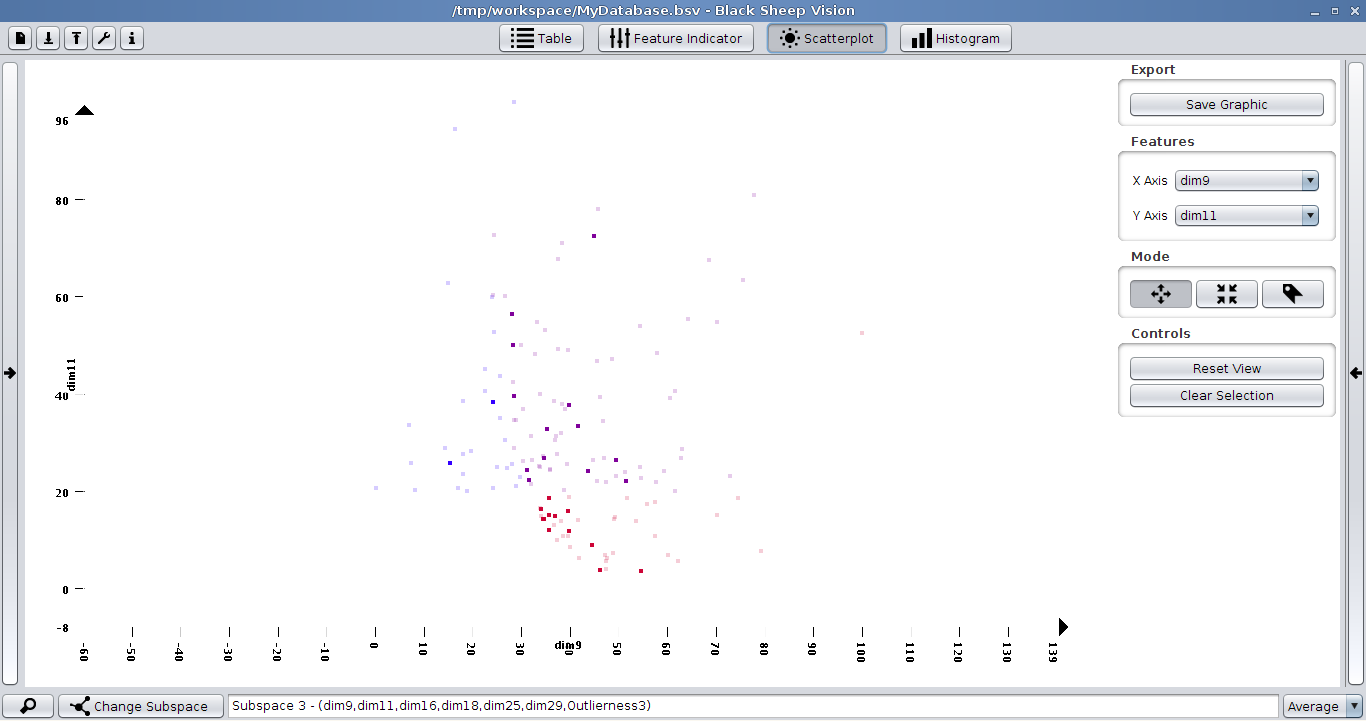
\includegraphics[width=16cm]{images/bsv/Scatterplot.png}
  \caption{Scatterplot}
  \label{fig:scatterplot}
\end{figure}

\subsection{Functionality}
\begin{tabular}{p{0.2\linewidth}p{0.7\linewidth}}
  \color{fancy}Feature & \color{fancy}Usage \\ \hline
  Display & The Scatterplot visualizes values of two features at a time. \\ \hline
  Control & On the right side you find the control menu, which lets you export the current view (e.g. as a \textbf{.svg}), specify the two features to plot or set the mode of the view. \\ \hline
  Modes & There are three different modes: move, zoom, and select. The move mode acts as default and lets you move the plot. The zoom mode lets you zoom in on a specific position. The select mode offers a tool for selecting an area of values. \\ \hline
  Select & You are able to select areas in this view by using the select mode. To discard all selections, you have to click the clear selection button, at the bottom of the control menu. \\ \hline
\end{tabular}

\subsection{Shortcuts}
\begin{center}
  \begin{spacing}{2.5}
  \begin{tabular}{c|l}
    \color{fancy}Shortcut & \color{fancy}Function\\
    \hline\hline
    \Ctrl + \keystroke{J} & Activates the move mode.\\
    \Ctrl + \keystroke{K} & Activates the zoom mode.\\
    \Ctrl + \keystroke{L} & Activates the select mode.\\
    \Ctrl + \keystroke{S} & Activates the select mode.\\
    \Ctrl + \keystroke{R} & Resets the selection.\\
  \end{tabular}
  \end{spacing}
\end{center}
